
\pagebreak
\section{Debugging}
If you've been writing perfect Matlab code up to this point... congratulations.
 But eventually you're likely to encounter a bug in you code.
 The graphical nature of the editor, and the interpreted nature of the code allows for easy debugging.

\subsection{Breakpoints}
You can enable a breakpoint by clicking on the small dash next to your code.
 This puts a red circle next to that line.
 The next time your code runs, it will stop right before executing that line.

\begin{figure}[ht!]
\centering
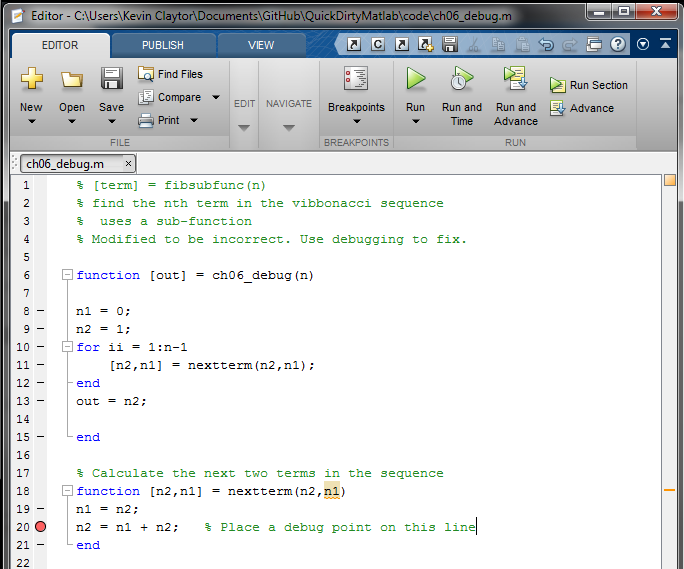
\includegraphics[width=90mm]{img/debug1.png}
\caption{Clicking on a tic-mark next to the line sets a debug point at that location.}
\label{guiload}
\end{figure}

\begin{figure}[ht!]
\centering
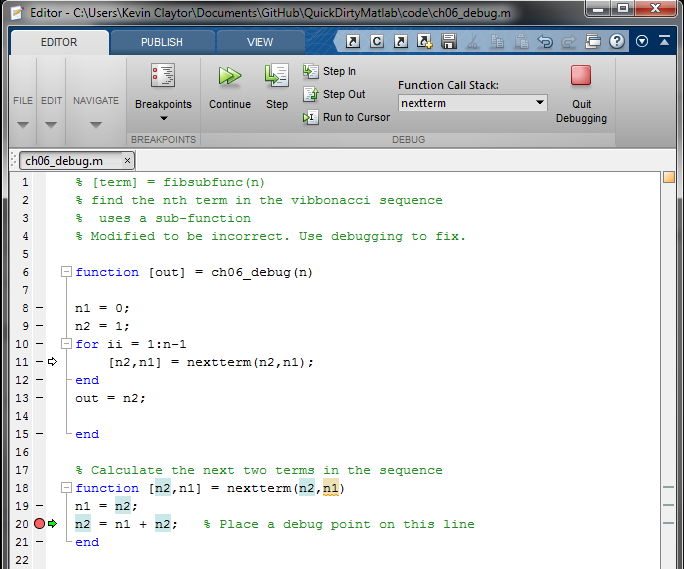
\includegraphics[width=90mm]{img/debug2.png}
\caption{When the function is called and the breakpoint reached, Matlab stops and presents you with the debugging view. Several of the commands described in the next section have graphical representations in this view.}
\label{guiload}
\end{figure}

\pagebreak
\subsection{Debug Commands}
\label{subsec:debugfile}
You can then use the step and continue commands to move through your code, investigating variable values as you go.
 Variable values are restricted to the workspace they appear in.
 You've already seen the workspace in the main window - your variables live there.
 Each function gets its own workspace.

\begin{center}
    \begin{tabular}{ | l | p{7cm} |}
    \hline Command & Description \\ \hline
    dbstep & Step to the next line in the code. \\ \hline
    dbcont & Continue to the next debug point. \\ \hline
    dbstack & Display all the function calls that got us to the current location. \\ \hline
    dbup & Move up into the caller's workspace. \\ \hline
    dbdown & Move down into the called function's workspace. \\ \hline
    dbquit & Quit debugging and return to the main workspace without evaluating any more code. \\ \hline
    who & List variables in current workspace. \\ \hline
    whos & List variables in workspace along with their dimensions, size in memory, and any atributes. \\ \hline
    which X & Can be used to investigate if X is a variables (says so) or a functions (returns the path to the function). \\ \hline
    \end{tabular}
\end{center}

The following code is a modified version of the fibsubfunc.m introduced in Chapter 4.
 There is an error in the subfunction that returns the next steps in the sequence.
 Use debugging to investigate it.

\begin{quote}
 \verbatiminput{code/ch06_debug.m}
\end{quote}

\pagebreak
\subsection{Waitbar}
Sometimes your code isn't broken, but just takes awhile to run.
 You can use the waitbar command to visualize the progress easially.

\begin{quote}
 \verbatiminput{code/ch06_waitbar.m}
\end{quote}
